\documentclass[12pt]{article}

\usepackage[margin=1.1in]{geometry}
\usepackage{amsmath,amssymb,amsthm}
\usepackage{graphicx}
\usepackage{booktabs}
\usepackage{hyperref}
\usepackage{xcolor}
\usepackage{natbib}
\usepackage{microtype}
\usepackage{caption}
\usepackage{subcaption}

\captionsetup{font=small, labelfont=bf}

\hypersetup{colorlinks=true, linkcolor=blue!70!black, citecolor=blue!70!black, urlcolor=blue!70!black}

\newcommand{\gam}{\gamma}
\newcommand{\ghat}{\hat{\gamma}}
\newcommand{\gGS}{\gamma_{\mathrm{GS}}}
\newcommand{\Hv}{\mathbf{h}}
\newcommand{\dtau}{\delta\tau}
\newcommand{\RMAE}{\mathrm{MAE}}

\title{\textbf{Trajectory Self-Supervised Learning for\\
Sample-Efficient Quantum Ground State Prediction}}

\author{Wenhao He\\
\small Massachusetts Institute of Technology\\
\small \texttt{wenhaohe@mit.edu}}

\date{\today}

% ─────────────────────────────────────────────────────────────────────────────
\begin{document}
\maketitle

% ── Abstract ─────────────────────────────────────────────────────────────────
\begin{abstract}
Predicting ground-state properties of quantum many-body systems from a Hamiltonian
description is a central problem in condensed matter physics, quantum chemistry, and
materials science. Machine learning approaches offer a promising route, but their
practical impact is limited by the cost of generating labeled training data: each
labeled example requires a full, expensive quantum simulation.
We observe that iterative quantum solvers---imaginary-time evolution, power iteration,
variational optimization---naturally produce trajectories of intermediate quantum states
as a byproduct of their convergence.
These intermediate states are typically discarded, yet they carry rich information about
the energy landscape and ground-state structure.
We propose \emph{trajectory self-supervised learning} (trajectory SSL), which exploits
these free intermediate states as a pretraining signal before fine-tuning on a small
number of labeled ground states.
On the one-dimensional Hubbard model, trajectory SSL achieves approximately $1.7\times$
lower prediction error compared to supervised learning on the final states alone,
at identical simulation budget.
The improvement persists out-of-distribution: models trained on the metallic regime
($U/t\!\in\![0,6]$) and evaluated on the strongly-correlated Mott insulator regime
($U/t\!\in\![6,10]$) show no degradation in the relative benefit.
Through a controlled ablation, we show that the gain has two components:
(i) learning the distribution of physical density matrices from diverse
intermediate-state samples, and (ii) an additional contribution from the
temporal ordering of the trajectory, which encodes the directional approach to
the ground state.
The method is robust to the choice of convergent dynamics: power iteration
trajectories yield results nearly identical to imaginary-time evolution,
suggesting broad applicability to any iterative quantum solver.
\end{abstract}

% ── 1. Introduction ──────────────────────────────────────────────────────────
\section{Introduction}
\label{sec:intro}

Predicting the ground-state properties of strongly correlated quantum systems is
a fundamental challenge with broad implications for quantum materials, high-temperature
superconductivity, and quantum chemistry.
Exact methods such as exact diagonalization (ED) and density matrix renormalization
group (DMRG) provide accurate results but scale exponentially or polynomially in
system size, making them prohibitively expensive for large systems or high-throughput
screening.

Machine learning (ML) has emerged as a promising complement: given a dataset of
solved Hamiltonians, one can train a model to directly predict ground-state
properties of new Hamiltonians at negligible inference cost
\citep{carrasquilla2017machine, carleo2017solving, han2019solving}.
The central bottleneck, however, is data: each labeled training example requires
a full quantum simulation, limiting practical dataset sizes to tens or hundreds of
examples.

In this work we ask a simple question: \emph{can we extract more value from a
fixed number of quantum simulations?}
The answer lies in a resource that is routinely generated but almost universally discarded.
When an iterative solver converges to the ground state---through imaginary-time evolution,
DMRG sweeps, or variational optimization---it produces a trajectory of intermediate
quantum states.
This trajectory encodes how the system ``flows'' toward the ground state and carries
substantial information about the ground-state structure.
Yet standard supervised approaches use only the final state $\gGS$,
ignoring all intermediate information.

We propose \textbf{trajectory self-supervised learning} (trajectory SSL):
a two-stage training procedure that first pretrains a predictor
$f_\theta(\gam_t, H) \to \gam_{t+1}$ on consecutive pairs of intermediate states
(no labels required), and then fine-tunes the same model as
$f_\theta(\gam_0, H) \to \gGS$ on a small labeled dataset.
At equal simulation budget---the same $N$ Hamiltonians for both methods,
with one trajectory per Hamiltonian---trajectory SSL consistently outperforms
supervised learning on final states alone by approximately $1.7\times$
across all $N$ tested (Fig.~\ref{fig:main}).

Beyond the empirical improvement, we conduct a mechanistic analysis to understand
\emph{why} trajectory pretraining helps.
Through a shuffled-trajectory ablation, we decompose the gain into two components:
a $\sim\!33\%$ improvement from learning the statistical distribution of
physical density matrices, and an additional $\sim\!20\%$ from the temporal
ordering of trajectory steps, which reflects the directional dynamics toward
the ground state (Fig.~\ref{fig:mechanism}).
We further show that the method is robust to the algorithm used to generate
trajectories: power iteration, which converges to the ground state via a
completely different mathematical route, yields nearly identical performance.

Finally, we demonstrate that trajectory SSL generalizes out-of-distribution:
models trained exclusively on Hamiltonians in the metallic regime
($U/t \in [0, 6]$) and evaluated on the Mott insulator regime
($U/t \in [6, 10]$) show no degradation in the relative benefit (Fig.~\ref{fig:ood}).
This suggests that the pretrained representation captures universal features of
quantum dynamics rather than regime-specific patterns.

Our contributions are:
\begin{enumerate}
  \item We identify that intermediate states produced by iterative quantum solvers
    constitute a free, high-quality self-supervised training signal.
  \item We propose trajectory SSL, a simple two-stage approach that exploits this
    signal and achieves ${\sim}1.7\times$ sample efficiency improvement at equal
    simulation cost.
  \item Through controlled ablations we decompose the mechanism into (i) RDM
    distribution learning and (ii) directional dynamics, and show the method is
    algorithm-agnostic.
  \item We demonstrate out-of-distribution generalization across the
    Mott metal-insulator crossover.
\end{enumerate}

% ── 2. Background ────────────────────────────────────────────────────────────
\section{Background}
\label{sec:background}

\subsection{The 1D Hubbard model and one-particle reduced density matrix}

We study the one-dimensional Hubbard model with open boundary conditions on $L=6$
sites at half-filling ($N_\uparrow = N_\downarrow = L/2$):
\begin{equation}
  H = -\sum_{\langle ij\rangle,\sigma} t_{ij}\, c^\dagger_{i\sigma} c_{j\sigma}
      + \sum_i \varepsilon_i\, n_i
      + U \sum_i n_{i\uparrow} n_{i\downarrow},
\label{eq:hubbard}
\end{equation}
where $t_{ij}$ is the nearest-neighbor hopping amplitude, $\varepsilon_i$ is the
onsite potential, and $U$ is the on-site Coulomb repulsion.
To create a diverse training distribution, we sample random Hamiltonians with
$t_{ij} \sim \mathcal{U}[0.5, 1.5]$, $\varepsilon_i \sim \mathcal{U}[-0.5, 0.5]$,
and $U \sim \mathcal{U}[0, 8]$; the Hamiltonian is represented by the
13-dimensional vector $\Hv = (t_{01}, \ldots, t_{L-1,0},\,\varepsilon_0,\ldots,\varepsilon_{L-1},\,U)$.

The target observable is the \emph{one-particle reduced density matrix} (1-RDM):
\begin{equation}
  \gam_{ij,\sigma} = \langle \psi_{\mathrm{GS}} | c^\dagger_{i\sigma} c_{j\sigma} | \psi_{\mathrm{GS}} \rangle,
\label{eq:rdm}
\end{equation}
organized as a $(2L \times 2L)$ matrix $\gam \in \mathbb{R}^{12\times 12}$.
The 1-RDM encodes all single-particle properties including the kinetic energy
$E_\mathrm{kin} = -\sum_{\langle ij\rangle,\sigma} t_{ij}(\gam_{ij} + \gam_{ji})$,
site occupations, and hopping correlations.

Ground states are computed by exact diagonalization (ED) of the Hilbert space
(dimension $\binom{L}{L/2}^2 = 400$).

\subsection{Imaginary-time evolution}

Imaginary-time evolution provides a standard route to the ground state from an
arbitrary initial state $|\psi_0\rangle$:
\begin{equation}
  |\psi(\tau)\rangle = \frac{e^{-\tau H} |\psi_0\rangle}{\| e^{-\tau H} |\psi_0\rangle \|}.
\label{eq:imag_time}
\end{equation}
As $\tau \to \infty$, $|\psi(\tau)\rangle \to |\psi_{\mathrm{GS}}\rangle$ (assuming
$\langle\psi_0|\psi_{\mathrm{GS}}\rangle \neq 0$).
We discretize with step $\dtau = 0.1$ and collect the 1-RDM at each step,
yielding a trajectory $(\gam_0, \gam_{\dtau}, \gam_{2\dtau}, \ldots, \gam_{T\dtau})$
with $T=30$ steps.
The intermediate states $\gam_t$ are generated as a byproduct of finding $\gGS$
and are the raw material for our self-supervised pretraining.

\subsection{Related work}

\paragraph{ML for quantum many-body systems.}
Neural network quantum states~\citep{carleo2017solving} and supervised learning
of Hamiltonian-to-property maps~\citep{han2019solving, roth2023group} have achieved
strong results on specific system classes.
Transfer learning across Hamiltonian families has been explored~\citep{zen2020transfer},
but typically requires target-domain fine-tuning data.
Our approach differs in that we exploit the \emph{dynamics within a single simulation}
rather than transferring across systems.

\paragraph{Self-supervised learning.}
SSL has driven advances in vision~\citep{chen2020simple} and language~\citep{devlin2019bert}
by learning representations from unlabeled data.
In scientific ML, SSL has been applied to molecular dynamics
trajectories~\citep{hu2021forcenet} and protein structures~\citep{jumper2021alphafold}.
Our work applies the SSL paradigm to quantum many-body trajectories, exploiting the
physical structure of imaginary-time flow as the pretraining objective.

\paragraph{Data efficiency in quantum simulation.}
Active learning~\citep{smith2018less} and Bayesian optimization have been used
to reduce the number of required simulations.
These approaches select which simulations to run; our approach instead extracts
more information from the simulations already run.

% ── 3. Method ────────────────────────────────────────────────────────────────
\section{Method}
\label{sec:method}

\subsection{Model architecture}

We parameterize the predictor as a \emph{DeltaPredictor}:
\begin{equation}
  f_\theta(\gam, H) = \gam + \mathrm{MLP}_\theta\bigl([\mathrm{vec}(\gam);\, \hat{\Hv}]\bigr),
\label{eq:model}
\end{equation}
where $\mathrm{vec}(\gam) \in \mathbb{R}^{144}$ is the flattened 1-RDM,
$\hat{\Hv} = (\Hv - \mu_H)/\sigma_H$ is the standardized Hamiltonian vector,
and $\mathrm{MLP}_\theta$ is a 4-layer network with hidden dimension 256, LayerNorm,
and GELU activations.
The output is symmetrized as $\tfrac{1}{2}[f + f^\top]$ to preserve the Hermitian
property of the 1-RDM.
The residual formulation biases the network toward small updates, which is
appropriate for both the pretraining task ($\gam_t \to \gam_{t+1}$ is a small step)
and fine-tuning (starting from $\gam_0$, the initial guess).

\subsection{Stage 1: Trajectory pretraining}

Given $N$ Hamiltonians sampled from the training pool, each with one imaginary-time
trajectory $(\gam_0^{(i)}, \gam_1^{(i)}, \ldots, \gam_T^{(i)})$, we construct $NT$
consecutive pairs and minimize:
\begin{equation}
  \mathcal{L}_{\mathrm{pre}}(\theta) = \frac{1}{NT} \sum_{i=1}^N \sum_{t=0}^{T-1}
  \bigl\| f_\theta(\gam_t^{(i)}, H^{(i)}) - \gam_{t+1}^{(i)} \bigr\|_F^2.
\label{eq:pretrain_loss}
\end{equation}
This objective asks the model to predict the next step of imaginary-time evolution,
purely from the current density matrix and the Hamiltonian---no ground-state labels.
Training uses AdamW with cosine learning-rate decay for 200 epochs.

\subsection{Stage 2: Supervised fine-tuning}

The pretrained model is then fine-tuned on the same $N$ labeled pairs
$\{(H^{(i)}, \gGS^{(i)})\}_{i=1}^N$:
\begin{equation}
  \mathcal{L}_{\mathrm{ft}}(\theta) = \frac{1}{N}\sum_{i=1}^N
  \bigl\| f_\theta(\gam_0, H^{(i)}) - \gGS^{(i)} \bigr\|_F^2,
\label{eq:ft_loss}
\end{equation}
where $\gam_0$ is a fixed canonical initial state (uniform diagonal:
$(\gam_0)_{ii} = N_\sigma/L$).
Fine-tuning uses AdamW with a smaller learning rate for 500 epochs.

\subsection{Baseline: endpoint-only supervised learning}

The endpoint-only baseline trains a fresh model from random initialization
directly on $\mathcal{L}_\mathrm{ft}$ using the same $N$ labeled pairs.
This corresponds to standard supervised learning without any trajectory data.

\subsection{Equal-budget guarantee}

The key fairness condition: both methods are given the same $N$ Hamiltonians,
with one imaginary-time trajectory per Hamiltonian (N\_TRAJ$=1$).
Running the trajectory solver produces the full sequence
$(\gam_0, \ldots, \gam_T, \gGS)$ in a single pass.
Endpoint-only uses only $\gGS$; trajectory SSL uses all $T+1$ intermediate states.
No additional quantum simulations are required.

% ── 4. Experiments ───────────────────────────────────────────────────────────
\section{Experiments}
\label{sec:experiments}

\subsection{Setup}

\paragraph{Data.}
300 Hamiltonians of the form~\eqref{eq:hubbard} are generated:
200 form the training pool, 100 are held out as a fixed test set.
Ground states and trajectories are computed by ED.

\paragraph{Evaluation.}
We report mean absolute error (MAE) between predicted and true 1-RDM:
$\RMAE = \frac{1}{N_\mathrm{test}} \sum_i \|\ghat_{\mathrm{GS}}^{(i)} - \gGS^{(i)}\|_1 / (2L)^2$.
Results are averaged over 5 random seeds (different $N$-sample draws from the pool);
error bars show $\pm 1$ standard deviation.

\subsection{Main result: equal-budget comparison}
\label{sec:main}

Figure~\ref{fig:main} shows MAE versus simulation budget $N$
for endpoint-only and trajectory SSL, for $N \in \{5, 10, 20, 50, 100, 200\}$.
Trajectory SSL consistently outperforms endpoint-only at every $N$,
with an improvement factor of approximately $1.7\times$ that is
remarkably stable across the full range.

\begin{table}[h]
\centering
\small
\caption{MAE of predicted $\gGS$ at equal simulation budget.}
\label{tab:main}
\begin{tabular}{ccccc}
\toprule
$N$ & Endpoint-only & Trajectory SSL & Improvement \\
\midrule
5   & $0.150 \pm 0.013$ & $0.105 \pm 0.008$ & $\times 1.43$ \\
10  & $0.121 \pm 0.004$ & $0.077 \pm 0.004$ & $\times 1.57$ \\
20  & $0.094 \pm 0.006$ & $0.053 \pm 0.003$ & $\times 1.77$ \\
50  & $0.047 \pm 0.002$ & $0.026 \pm 0.001$ & $\times 1.81$ \\
100 & $0.022 \pm 0.001$ & $0.012 \pm 0.000$ & $\times 1.83$ \\
200 & $0.011 \pm 0.000$ & $0.006 \pm 0.000$ & $\times 1.83$ \\
\bottomrule
\end{tabular}
\end{table}

The practical implication is direct: achieving a target accuracy with
trajectory SSL requires approximately half as many expensive quantum simulations
as endpoint-only supervised learning.

\subsection{Out-of-distribution generalization}
\label{sec:ood}

To test generalization to qualitatively different physics, we train both methods
on pool Hamiltonians with $U/t \in [0, 6]$ (metallic to weakly correlated regime)
and evaluate on test Hamiltonians with $U/t \in [6, 10]$ (strongly-correlated
Mott insulator regime), which were never seen during training.

Figure~\ref{fig:ood} shows that the ${\sim}1.7\times$ improvement is preserved
out-of-distribution: trajectory SSL achieves $\times 1.3$--$1.8$ across all $N$,
nearly identical to the in-distribution result.
This indicates that trajectory pretraining learns representations that generalize
across the metal-insulator crossover, capturing features of imaginary-time dynamics
that are universal rather than regime-specific.

\subsection{Mechanistic analysis}
\label{sec:mechanism}

Figure~\ref{fig:mechanism} decomposes the improvement via two ablations.

\paragraph{Panel (a): Algorithm robustness.}
We replace imaginary-time trajectories with power-iteration trajectories:
\begin{equation}
  |\psi_{k+1}\rangle = \frac{(cI - H)|\psi_k\rangle}{\|(cI - H)|\psi_k\rangle\|},
  \quad c = 20,
\end{equation}
which also converges to the ground state (the dominant eigenvector of $cI - H$)
via a completely different mathematical route.
Power-iteration SSL achieves nearly identical performance to imaginary-time SSL
at all $N$ (Table~\ref{tab:mechanism}), confirming that the benefit is not specific
to the imaginary-time operator but arises from any convergent dynamics.

\paragraph{Panel (b): Role of temporal ordering.}
We introduce a \emph{shuffled SSL} baseline that uses the same $NT$ intermediate-state
frames as trajectory SSL, but randomly pairs them as $(\gam_i, \gam_j)$ with
$j \neq i$ sampled uniformly---breaking the temporal structure while preserving
the set of RDM values seen.

Shuffled SSL outperforms endpoint-only (e.g., $0.064$ vs $0.096$ at $N=20$),
confirming that simply exposing the model to diverse physical density matrices
provides a useful inductive bias about the RDM output space.
However, ordered trajectory SSL further outperforms shuffled SSL
($0.053$ vs $0.064$ at $N=20$, $\sim\!17\%$ additional gain),
demonstrating that the temporal ordering---the directional approach toward
$\gGS$---encodes information beyond the marginal RDM distribution.

\begin{table}[h]
\centering
\small
\caption{MAE at $N=20$, decomposing the trajectory SSL gain.}
\label{tab:mechanism}
\begin{tabular}{lcc}
\toprule
Method & MAE ($N=20$) & vs.\ endpoint \\
\midrule
Endpoint-only        & $0.096$ & $\times 1.00$ \\
Shuffled SSL         & $0.064$ & $\times 1.50$ \\
Power-iteration SSL  & $0.057$ & $\times 1.68$ \\
Imaginary-time SSL   & $0.053$ & $\times 1.81$ \\
\bottomrule
\end{tabular}
\end{table}

Taken together, the two panels support the following picture:
the total gain (${\sim}1.8\times$) arises roughly two-thirds from
learning the distribution of physical density matrices (captured by shuffled SSL)
and one-third from the directional information in the temporal ordering.
Both components transfer out-of-distribution, and neither requires ground-state labels.

% ── 5. Discussion ────────────────────────────────────────────────────────────
\section{Discussion}
\label{sec:discussion}

\paragraph{Broader applicability.}
Our results suggest a general principle: \emph{any iterative quantum solver that
produces a sequence of intermediate states can serve as a source of self-supervised
training data}.
This encompasses DMRG sweeps (where intermediate bond-dimension states are available),
quantum Monte Carlo Markov chains (where walker configurations form a trajectory),
and variational optimization (where parameter updates trace a path in state space).
In each case, the intermediate states are generated as a byproduct of the solver
and are currently discarded.

\paragraph{Limitations and future work.}
The present study is limited to small systems ($L=6$, exact diagonalization)
and the 1-RDM as the target observable.
Extending to larger systems requires either a more expressive model architecture
(e.g., equivariant networks) or a different 1-RDM parameterization, as the
flat MLP input grows as $O(L^2)$.
Predicting higher-order correlators (2-RDM, spectral functions) would require
extending the output representation but not the core pretraining principle.
We also note that the equal-budget comparison fixes the number of Hamiltonians;
exploring the trade-off between Hamiltonian diversity and trajectory length
is an interesting direction.

\paragraph{Connection to score-based methods.}
The pretraining objective---predicting $\gam_{t+1}$ from $(\gam_t, H)$---is
structurally similar to score matching~\citep{hyvarinen2005estimation} and
denoising diffusion~\citep{ho2020denoising}.
Imaginary-time evolution can be viewed as a deterministic diffusion process
in Hilbert space that ``denoises'' the initial state toward the ground state.
This connection may open routes to applying diffusion-model techniques
to quantum state estimation.

% ── 6. Conclusion ────────────────────────────────────────────────────────────
\section{Conclusion}
\label{sec:conclusion}

We have introduced trajectory self-supervised learning, a simple method that
exploits the intermediate quantum states produced by iterative solvers as free
pretraining data.
On the 1D Hubbard model, trajectory SSL reduces the number of labeled simulations
required to reach a given prediction accuracy by approximately $2\times$,
at no additional computational cost---the trajectory is already generated as
a byproduct of computing the ground state.
The improvement is robust across simulation budgets, out-of-distribution
(across the Mott metal-insulator transition), and across different convergent
dynamics (imaginary-time evolution and power iteration).
Mechanistic ablations show that the gain has two separable components:
learning the distribution of physical density matrices, and learning the
directional dynamics of convergence.

We believe this observation---that solvers already generate the data needed for
better generalization---has practical value for workflows where quantum simulations
are expensive, and theoretical interest as a connection between iterative
numerical methods and self-supervised representation learning.

% ── References ───────────────────────────────────────────────────────────────
\bibliographystyle{abbrvnat}
\bibliography{refs}

% ── Figures ──────────────────────────────────────────────────────────────────
\clearpage

\begin{figure}[h]
  \centering
  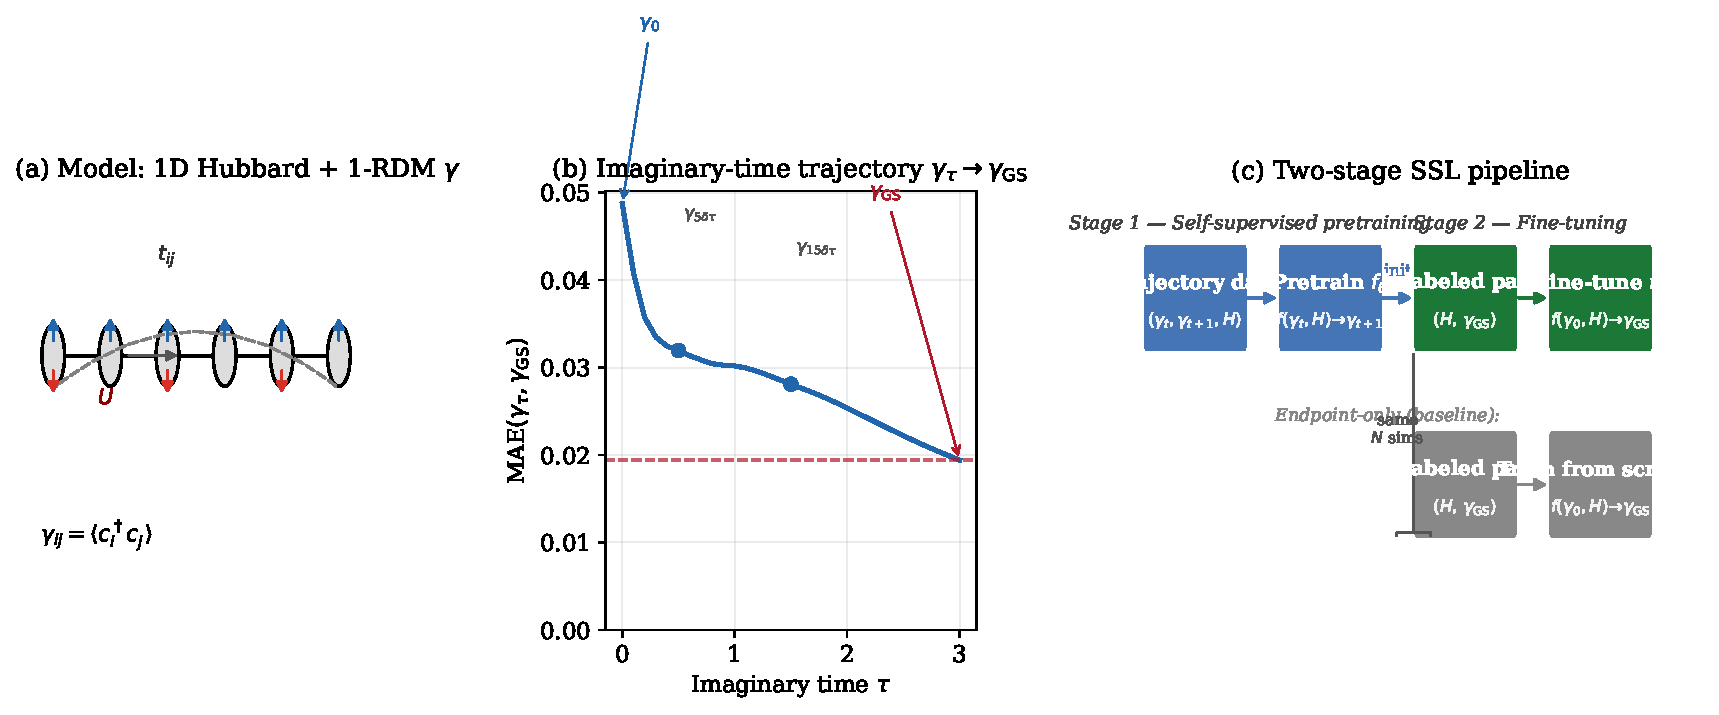
\includegraphics[width=\textwidth]{../fig1/fig1_schematic.pdf}
  \caption{\textbf{Trajectory SSL overview.}
  (a) We study the 1D Hubbard model with random hopping $t_{ij}$, onsite disorder
  $\varepsilon_i$, and interaction $U$. The target observable is the one-particle
  reduced density matrix (1-RDM) $\gam_{ij} = \langle c^\dagger_i c_j \rangle$.
  (b) Imaginary-time evolution $e^{-\tau H}|\psi_0\rangle/\|{\cdot}\|$ produces a
  trajectory $\gam_0 \to \gam_\tau \to \cdots \to \gGS$ that converges to the
  ground state; these intermediate states are free byproducts of the solver.
  (c) Stage~1 (blue): pretrain predictor $f_\theta(\gam_t, H) \to \gam_{t+1}$
  on $N$ trajectory pairs---no ground-state labels required.
  Stage~2 (green): fine-tune $f_\theta(\gam_0, H) \to \gGS$ on $N$ labeled examples.
  Both stages use the same $N$ Hamiltonians (equal simulation budget).
  The endpoint-only baseline (gray) trains from scratch on final states only.}
  \label{fig:schematic}
\end{figure}

\begin{figure}[h]
  \centering
  
\includegraphics[width=0.62\textwidth]{../fig2/fig1_exp1.pdf}
  \caption{\textbf{Main result: trajectory SSL reduces labeled data requirements
  by ${\sim}1.7\times$.}
  MAE of predicted $\gGS$ vs.\ number of simulations $N$ for endpoint-only
  (gray, dashed) and trajectory SSL (blue, solid).
  Both methods use the same $N$ Hamiltonians with one trajectory per Hamiltonian
  (equal simulation budget).
  Trajectory SSL achieves approximately $1.7\times$ lower error across all $N$,
  peaking at $\times 1.83$ for $N \geq 50$.
  Error bars: $\pm 1$ s.d.\ over 5 random seeds.}
  \label{fig:main}
\end{figure}

\begin{figure}[h]
  \centering
  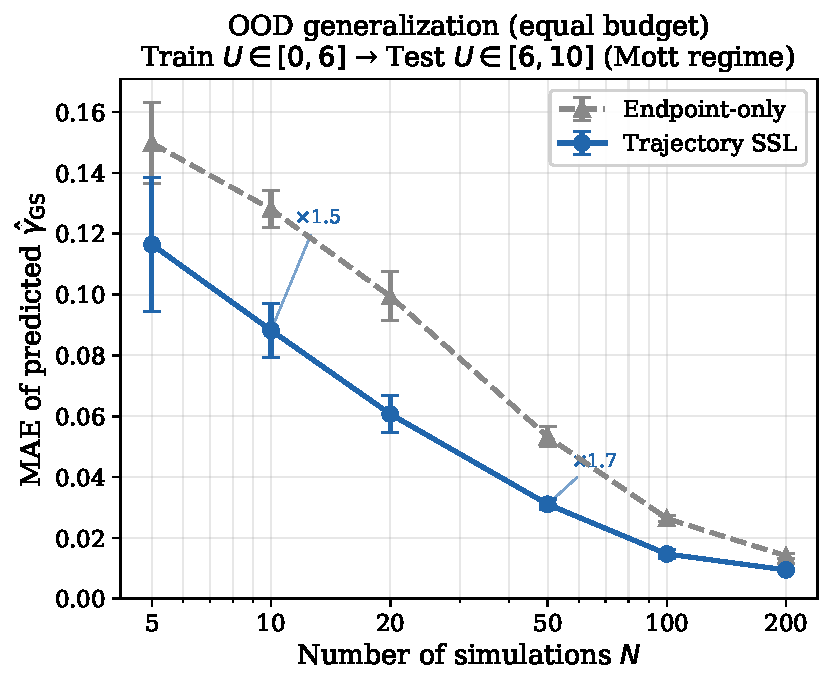
\includegraphics[width=0.62\textwidth]{../fig4_ood/fig4_ood.pdf}
  \caption{\textbf{OOD generalization to the Mott insulator regime.}
  Same experiment as Fig.~\ref{fig:main} but with training pool restricted to
  $U/t \in [0, 6]$ (metallic regime) and test set drawn from
  $U/t \in [6, 10]$ (strongly-correlated Mott insulator regime, never seen
  during training).
  The ${\sim}1.7\times$ improvement is preserved out-of-distribution
  ($\times 1.3$--$1.8$ across all $N$), indicating that trajectory SSL
  learns representations that generalize across qualitatively different
  physical regimes.
  Error bars: $\pm 1$ s.d.\ over 5 random seeds.}
  \label{fig:ood}
\end{figure}

\begin{figure}[h]
  \centering
  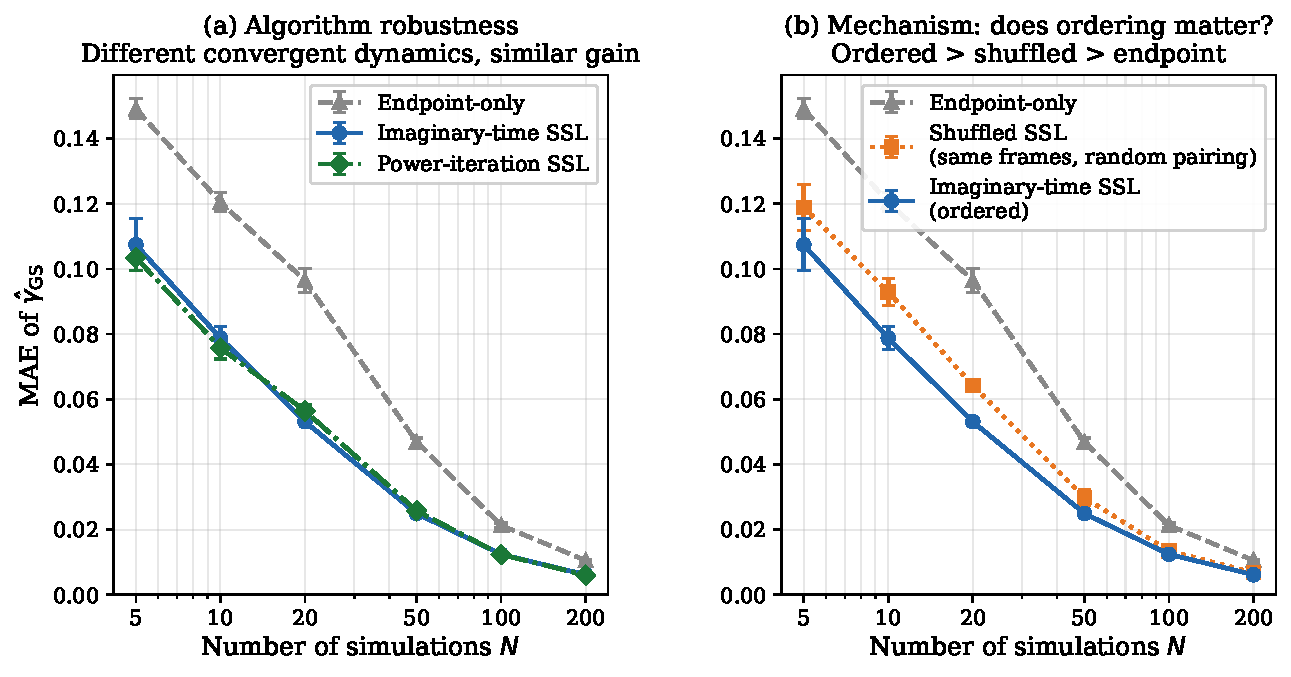
\includegraphics[width=\textwidth]{../fig5/fig5_two_panel.pdf}
  \caption{\textbf{Mechanistic analysis of trajectory SSL.}
  (a) \emph{Algorithm robustness}: endpoint-only (gray), imaginary-time SSL (blue),
  and power-iteration SSL (green). Power iteration uses the recurrence
  $(cI - H)|\psi\rangle/\|{\cdot}\|$ with $c=20$, a completely different
  convergent algorithm. The near-identical performance of imaginary-time and
  power-iteration SSL confirms that the benefit is not specific to imaginary-time
  evolution.
  (b) \emph{Role of temporal ordering}: endpoint-only (gray), shuffled SSL---same
  $\gam_t$ frames randomly re-paired (orange), and imaginary-time SSL (blue).
  Shuffled SSL $>$ endpoint-only: diverse RDM samples alone provide a useful
  inductive bias. Ordered SSL $>$ shuffled: the temporal ordering
  encodes additional directional information ($\sim\!17\%$ further gain at $N=20$).
  Error bars: $\pm 1$ s.d.\ over 5 random seeds.}
  \label{fig:mechanism}
\end{figure}

\end{document}
